\chapter{LITERATURE REVIEW}

%(20\% of Report Length)

% a. Must be paraphrased without plagiarizing

% b. Must include the base papers\cite{Adhikari2020Dec}, and support the rationale of the project

% c. Must highlight the strengths and shortcomings of the works performed by other authors
There are very few NER works available in the literature for Nepali (Bam and Shahi 2014; Dey, Paul, and Purkayastha 2014; Singh, Padia, and Joshi 2019). The first one is by Bam and Shahi (Bam and Shahi 2014) which utilized SVM to detect Person, Organization, Location, and Misc categories. They used word features as well as gazetteers including person, organization, location, middle name, verb, designation, and others. The SVM model was trained in one vs rest classification-cation setting. This first known model for NER in Nepali has several shortcomings: (a) it is not clear how the authors generated the training data set. The quality of the training data set is not reported either, (b) their work did not take context information into account while training the model, and (c) computing features like this hinder the scale-ability of the NER work \cite{1}.\\ 

The second work is by Dey and Pmkayastha (Dey, Paul, and Purkayastha 2014) who used the Hidden Markov Model with the n-gram technique for extracting POS tags. POS tags with a common noun, proper noun, or combination of both are combined, then a gazetteer list as a look-up table to identify the named entities. Results are reported for 750 sentences corresponding to Person, Location, Number, Organization, Currency, and Quantifier. This is a very Plim-live work that does not describe how the training exam-plus are obtained and used. The proposed Methodology is very vague \cite{2}.\\

The third work, and the most recent one, is by Singh et al. (Singh, Padia, and Joshi 2019) who studied NER in Nepali is the closest work to our work. The authors first collected sentences from daily newspapers and annotated three types of entities: Person, Location, and Organization. The authors then trained multiple neural models such as BiLSTM, BiLSTMCNN, BiLSTM-CRF, and BiLSTM-CNN-CRF with different word embedding. Although this work provides a data set (NepaliNER) publicly, the authors have not provided the annotation guideline nor conducted the human evaluation of the annotated corpus e.g. inter-rater reliability, making the data set less reliable. Furthermore, it does not provide separate train and test data sets, making it harder for other NER systems to be evaluated and compared \cite{3}.
\newpage
Mono vs Multilingual BERT: A Case Study in Hindi and Marathi Named Entity Recognition Performed by (Onkar Litake
, Maithili Sabane
, Parth Patil
, Aparna Ranade
and Raviraj Joshi-
Pune Institute of Computer Technology, Pune, Indian Institute of Technology Madras, Chennai
 L3Cube, Pune) 
 In this work, they have consider NER
for low-resource Indian languages like Hindi
and Marathi. The transformer-based models
have been used for NER tasks. By considering different variations of BERT like baseBERT, RoBERTa, and AlBERT and benchmark them on publicly available Hindi and
Marathi NER datasets and provide an exhaustive comparison of different monolingual and
multilingual transformer-based models and establish simple baselines currently missing in
the literature. They have shown that the monolingual
MahaRoBERTa model performs the best for
Marathi NER whereas the multilingual XLMRoBERTa performs the best for Hindi NER.
Also perform cross-language evaluation
and present mixed observations \cite{litake2022mono}.\\

Biomedical Named Entity Recognition with Multilingual BERT 
(Kai Hakala, Sampo Pyysalo)
Turku NLP Group, University of Turku, Finland. 
They have presented the approach of the Turku NLP
group to the PharmaCoNER task on Spanish
biomedical named entity recognition. Where they apply a CRF-based baseline approach and multilingual BERT to the task, achieving an Fscore of 88\% on the development data and
87\% on the test set with BERT. Their approach reflects a straightforward application
of a state-of-the-art multilingual model that is
not specifically tailored to either the language
nor the application domain \cite{hakala-pyysalo-2019-biomedical}.\\

Named-Entity Based Sentiment Analysis of Nepali News Media Texts
(Birat Bade Shrestha, Bal Krishna Bal)
Information and Language Processing Research Lab,
Department of Computer Science \& Engineering,
Kathmandu University, Dhulikhel, Kavre, Nepal. They have used news Media text for sentiment analysis. Their major
challenge with texts was the difficulty
in aligning the expressed opinions with the
concerned political leaders as this entails a
non-trivial task of named-entity
recognition and anaphora resolution. In
that work, their primary focus was on
developing a Natural Language Processing
(NLP) pipeline involving a robust NamedEntity Recognition followed by Anaphora
Resolution and then after alignment of the
recognized and resolved named-entities, in
that case, political leaders to the correct
class of opinions as expressed in the texts.
They visualize the popularity of the
politicians via the time series graph of
positive and negative sentiments as an
outcome of the pipeline. They had
achieved the performance metrics of the
individual components of the pipeline as
follows: Part of speech tagging – 93.06\%
(F1-score), Named-Entity Recognition –
86\% (F1-score), Anaphora Resolution –
87.45\% (Accuracy), Sentiment Analysis –
80.2\% (F1-score) \cite{bade-shrestha-bal-2020-named}.\\

NepBERTa: Nepali Language Model Trained in a Large Corpus
(Milan Gautam
, Sulav Timilsina
Palua.AI Ltd, UK ,Binod Bhattarai
Nepal Applied Mathematics and
Informatics Institute for research (NAAMII), Nepal). This work presents NepBERTa, a BERT-based Natural Language Understanding (NLU) model trained on the most extensive monolingual Nepali corpus.
They have collected a dataset of 0.8B words from 36
different popular news sites in Nepal and introduced the model. Their data set was 3 folds times
larger than the previous publicly available corpus. They evaluated the performance of NepBERTa in multiple Nepali-specific NLP tasks,
including Named-Entity Recognition, Content
Classification, POS Tagging, and Categorical
Pair Similarity. 
They have also introduce two different datasets for two new downstream tasks and
benchmark four diverse NLU tasks altogether. They bring all these four tasks under the firstever Nepali Language Understanding Evaluation (Nep-gLUE) benchmark \cite{timilsina-etal-2022-nepberta}.\\

A Survey on Deep Learning for Named Entity Recognition (Jing Li, Aixin Sun, Jianglei Han, and Chenliang Li). This survey indicates named entity recognition (NER) is the task to identify mentions of rigid designators from text belonging to predefined
semantic types such as person, location, organization etc. NER is the foundation for many natural language applications such as question answering, text summarization, and machine translation. Early NER systems got a huge success in achieving good performance with the cost of human engineering in designing domain-specific features and rules. In recent years, deep
learning, empowered by continuous real-valued vector representations and semantic composition through nonlinear processing, has
been employed in NER systems, yielding stat-of-the-art performance. In this paper, they provide a comprehensive review on existing
deep learning techniques for NER. They first introduce NER resources, including tagged NER corpora and off-the-shelf NER tools. Then, systematically categorize existing works based on a taxonomy along three axes: distributed representations for input, context
encoder, and tag decoder. Next, they survey the most representative methods for recent applied techniques of deep learning in new
NER problem settings and applications. Finally, they present readers with the challenges faced by NER systems and outline future
directions in this area \cite{li2020survey}.





\section{Existing Systems}
\vspace{10pt} % Adjust the value as needed
\subsection{displaCy}
displaCy is an example of an English name entity recognition system. The spaCy library offers an interactive visualization tool displaCy for Natural Language Processing (NLP) activities. It makes it possible to visualize named entities and syntactic dependencies in text data. Users can create dependency parse trees using displaCy that highlight the relationships between words and display the grammatical structure of phrases. It also offers visualizations for named entity recognition, emphasizing things like people, organizations, places, and dates with various labels or colors. The linguistic characteristics of text data can be better understood by NLP practitioners and scholars thanks to this web-based tool’s support for many languages and customizable choices. Users can examine and explore NLP task outputs more effectively and intuitively by merging displaCy with spaCy \cite{displaCy}.
\\
\\

\begin{figure}[H]
\centering

\includegraphics[width=0.4\linewidth]{img/Graphics/displacy2.jpg}
%\caption[System Block Diagram]{DisplaCy}
%\label{fig:SystemBlockDiagram.png}

\end{figure}

\begin{figure}[H]
\centering
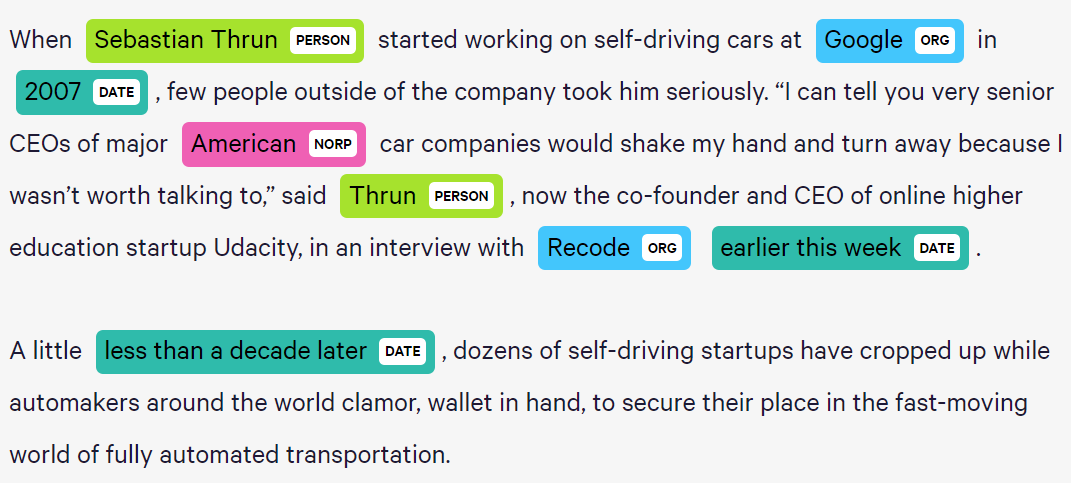
\includegraphics [scale=0.75 ]{img/Graphics/displacy3.png}
\caption[DisplaCy]{DisplaCy \textit{(Source: \href{https://explosion.ai/about}{Explosion, 2024})}}
\label{fig:DisplaCy.png}

\end{figure}

\subsection{Indic Named Entity Recognition (NER)}

Indic Named Entity Recognition (NER) is a natural language processing (NLP) task that involves identifying and classifying entities (such as names of people, locations, organizations, etc.) in text written in Indic languages. The term "Indic" refers to a group of languages spoken in the Indian subcontinent, which includes languages like Hindi, Bengali, Telugu, Tamil, and others.

Named Entity Recognition is crucial for understanding the structure and content of the text, as it helps in extracting meaningful information about specific entities mentioned in the text. Indic NER specifically focuses on the challenges posed by the linguistic characteristics of Indic languages.

Key aspects of Indic Named Entity Recognition:

\textbf{Diversity of Indic Languages}: Indic NER needs to account for the linguistic diversity among different Indic languages, each with its script, morphology, and syntactic structures.

\textbf{Morphological Complexity}: Indic languages often have complex word forms due to rich inflections and derivations. Effective NER models for Indic languages need to handle these morphological complexities.

\textbf{Script Variations}: Indic scripts vary across languages, and each script poses unique challenges for text processing. For example, Hindi uses the Devanagari script, while Bengali uses the Bengali script.

\textbf{Resource Scarcity} : Compared to widely studied languages like English, there may be limited labeled datasets and linguistic resources for Indic languages, making the development of accurate NER models more challenging.

Researchers and practitioners working on Indic NER often employ techniques like rule-based approaches, statistical models, and more recently, deep learning methods to address these challenges. The goal is to create models that can accurately identify and classify named entities in text written in Indic languages, supporting various applications such as information extraction, question answering, and language understanding in these diverse linguistic contexts \cite{mhaske2022naamapadam}.

\vspace{10pt}

\begin{figure}[H]
\centering
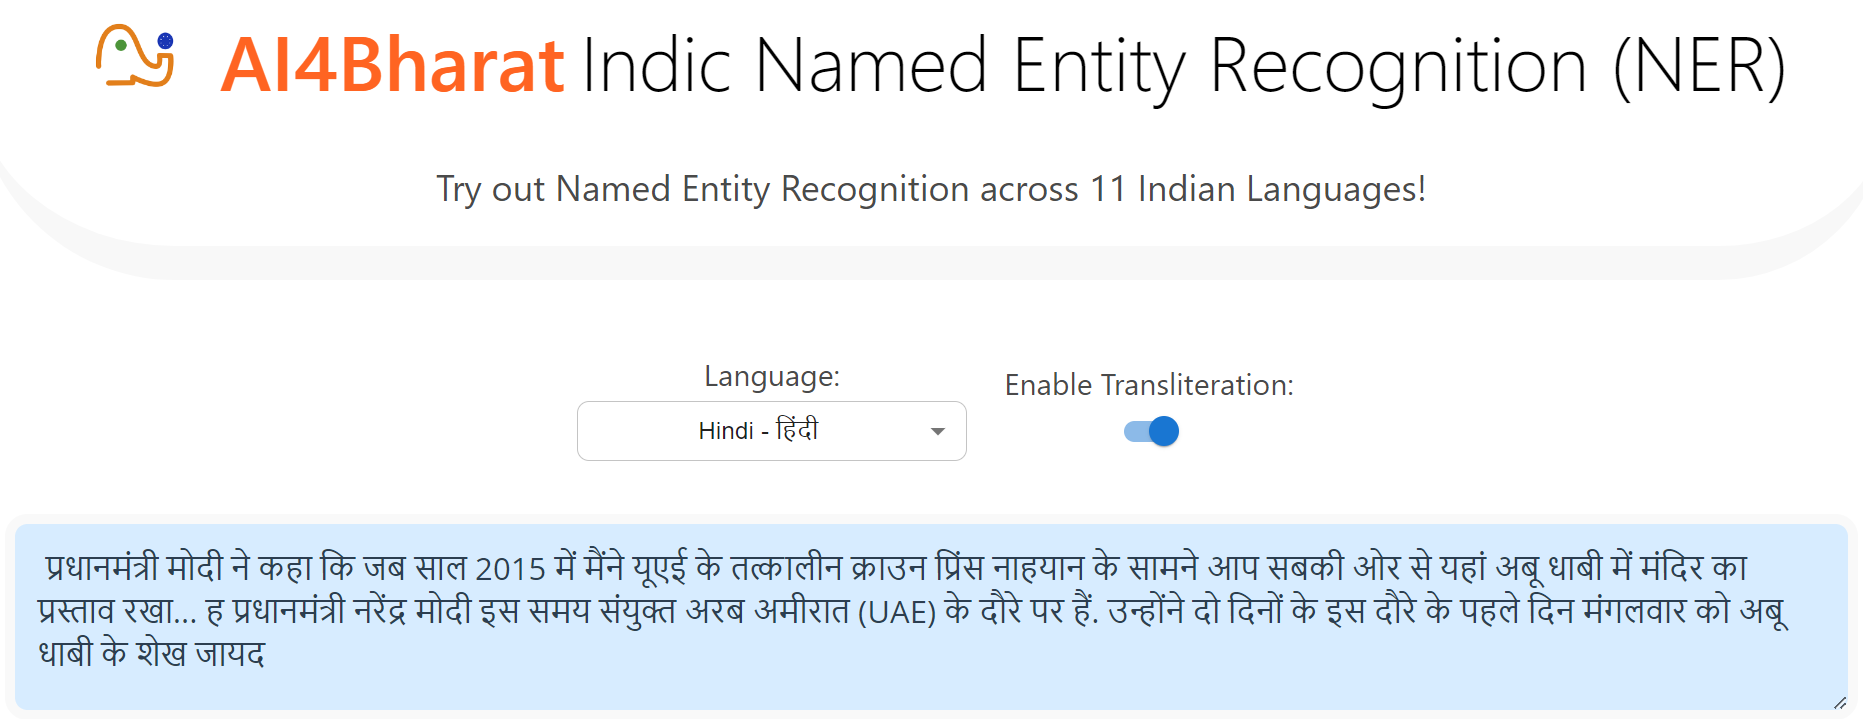
\includegraphics [scale=0.44 ]{img/ai4bharat/ai4bharat.png}
\caption[AI4Bharat
Indic NER With Input Section]{AI4Bharat Indic NER With Input Section \textit{(Source: \href{https://ai4bharat.iitm.ac.in/}{AI4Bharat, 2024})}}
\label{fig:DisplaCy.png}

\end{figure}

\begin{figure}[H]
\centering
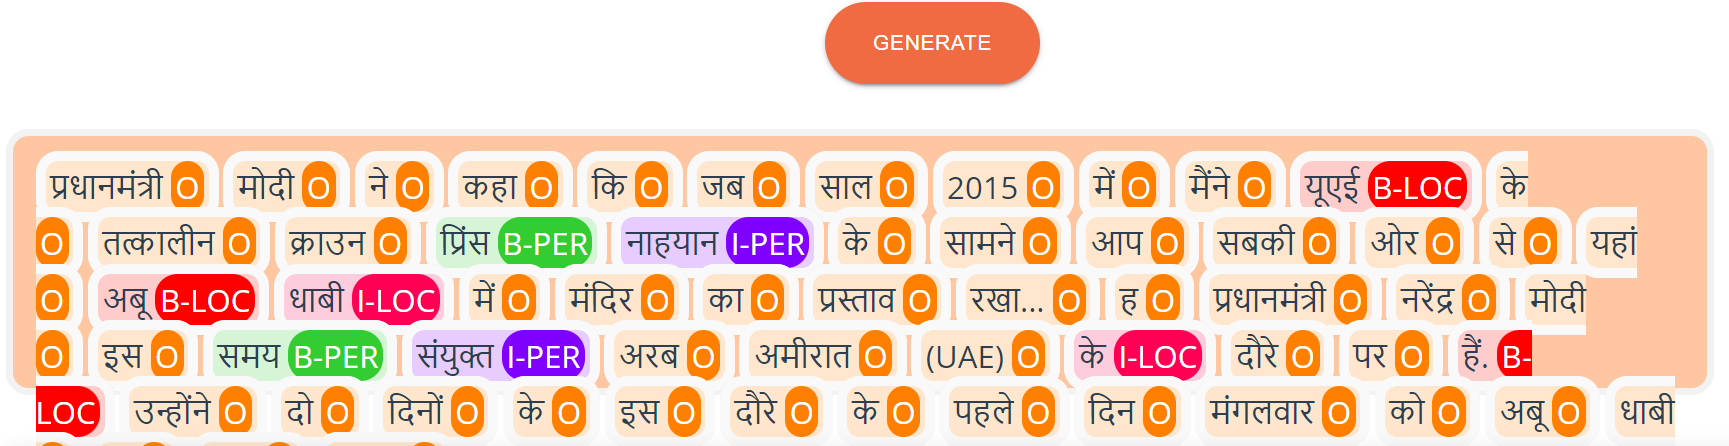
\includegraphics [scale=0.46 ]{img/ai4bharat/ai4bharat2.png}
\caption[AI4Bharat
Indic NER With Generated Named Entity sets]{AI4Bharat
Indic NER With Generated Named Entity sets \textit{(Source: \href{https://ai4bharat.iitm.ac.in/}{AI4Bharat, 2024})}}
\label{fig:DisplaCy.png}

\end{figure}



\subsection{DanfeNER}

DanfeNER - Named Entity Recognition in Nepali Tweets is a Named entity recognition system made by Nobal Niraula and Jeevan Chapagain. Twitter allows users to easily post tweets on any subject or event anytime, generating massive amounts of rich text content on diverse topics. Automated methods such as Named Entity Recognition (NER) are required to process the massive tweet data. Processing tweets, however, poses a special challenge as they are informal posts with incomplete context and often contain acronyms, hashtags, misspellings, abbreviations, and URLs due to length constraints. This NER system presents the first systematic study of NER in Nepali tweets corresponding to five different entity types: Person Name (PER), Location (LOC), Organization (ORG), Date (DAT), and Event (EVT). DanfeNER has good benchmark data sets for the low-resource language Nepali. DanfeNER contains 5,366 records and 3,463 entities in its train set and 2,301 records and 1,503 entities in its test set. Using this dataset benchmark of several state-of-the-art Nepali monolingual and multilingual transformer models, obtaining micro averaged F1scores up to 81\% \cite{Niraula_Chapagain_2023}.

\section{Proposed Systems}
Our Name Entity Recognition System is an online tool designed to extract name entities from given text documents. It is based on the Nepali and Devanagari text strings. It focuses on providing strong extraction and detection facilities enhancing the potential of the Nepali text format. Users can sign into the system to analyze and detect potential Name Entities, including personal names, locations, and organizations. The system uses an advanced transformer model -A bert-based-multilingual-cased pre-trained model. With the help of a trained model, the system assists users in detecting named entities of the Nepali language using natural language processing.

 